\section{Improved the SFC system}
\label{sec:sfc}

\url{gitolite@nedm.psi.ch:babySFC}

\textit{Overview}: Surrounding Field Compensation \cite{Franke2013, Rawlik2018a} system, or the \textbf{SFC}, is an important part of the n2EDM experimental setup. Its purpose is to sustain a magnetic field of a desired magnitude and direction in the measurement area. This goal is achieved by controlling the currents in a set of the magnetic coils \cite{Rawlik2018} in order to respond to the changes in the magnetic fields of the environment. The aim of the Feature \ref{sec:sfc} is similar to the one introduced in the Feature \ref{sec:rm-proxy}. SFC needed to be converted into a regular DAQ node that can be controlled over the SCPI connection and that can feed the COM handler with the experimental data in a compliant \cite{Bison2018} way and shape.

\subsection{SCPI interface}
\label{subsec:sfc_scpi}

\textit{Motivation}: we would like to replace an existing GUI control capabilities with a set of the SCPI commands in order to predictably govern the state of execution and the setup parameters of the SFC system.

\begin{figure}[h]
	\centering
	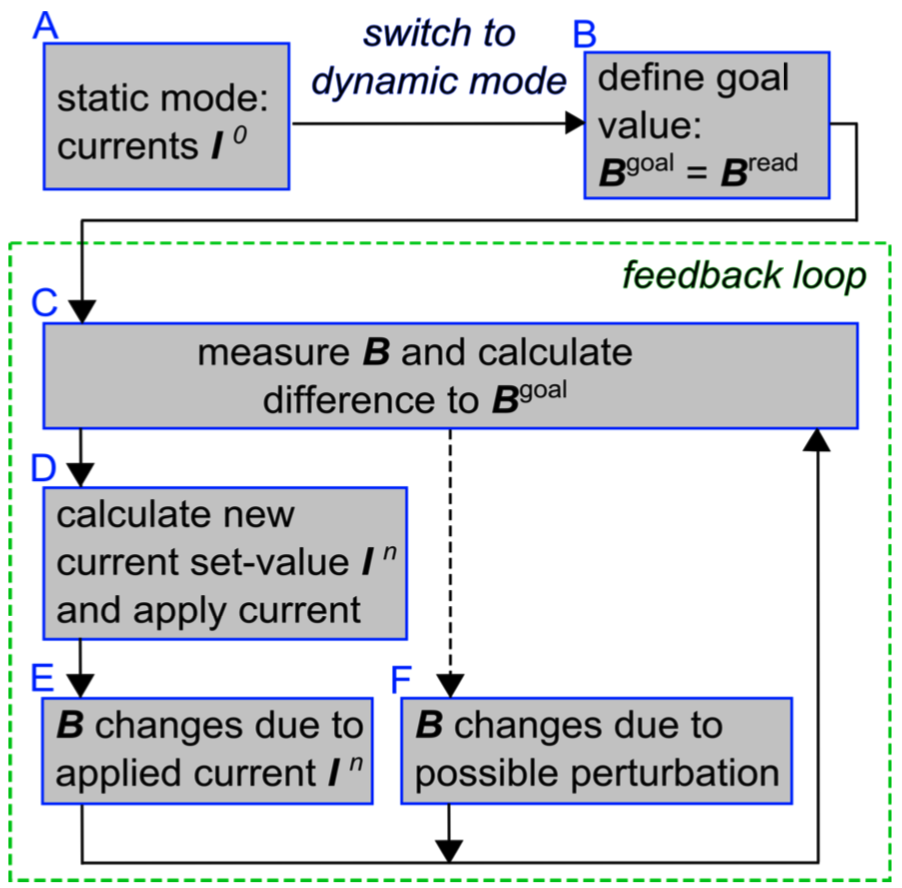
\includegraphics[width=\textwidth]{img/sfc_algorithm}
	\caption{Schematic structure of the SFC lifecycle taken from \cite{Franke2013}.}
	\label{fig:sfc_algorithm}
\end{figure}

\textit{Requirements}: as described in great details in \cite{Franke2013} the SFC system can run in either \texttt{STATIC} or \texttt{DYNAMIC} mode. While in \texttt{STATIC} the system is time-independent and fully characterised with $I^0$ which is a vector with every individual component defining a ratio of the immediate set current in the corresponding coil to the current at the nominal generated magnetic field. When switched to the \texttt{DYNAMIC} mode the new $I^n$ is recalculated on every iteration based on the difference between the expected and the measured fields. An overview of the SFC behaviour in the different modes can be found on the Figure \ref{fig:sfc_algorithm}.

We introduce the following 2 commands to control the experimental setup:
\begin{itemize}
	\item \texttt{MODE <STATIC|DYNAMIC>} that switches between the execution modes.
	\item{
		\texttt{COIL index, current} to modify the components of the $I^0$.
		\begin{itemize}
			\item \texttt{index}, required integer --- an index of the corresponding coil. The coil index itself is derived from the coil's position in the config file. Indices start with 1. Any index that is outside the $I^0$ boundaries is ignored and an error message is printed.
			\item \texttt{current}, required float --- a ratio of the current to be set to the maximal current. However at the moment there are no checks and one can set this value to be greater than 1 if desired.
		\end{itemize}
	}
\end{itemize}

\textit{Implementation details}: existing SFC software communicates with the main \texttt{babySFC.jl} module via a ZeroMQ connection. This endpoint was kept for the sake of the compatibility. However it is important to notice that these ZeroMQ messages simply contain the \textbf{name of the variable} and its new value to be set. Thus one needs to make sure that until the legacy scripts are properly modified to work with the SCPI commands it is necessary to keep the variable name that defines $I^0$ to be \texttt{staticI}.

\subsection{Data interface}
\label{subsec:sfc_data}

\textit{Motivation}: in the n2EDM DAQ system the COM handler is responsible for writing the data to the disk for the further analysis thus it is the job of the SFC to bundle it into a binary message and send the package over TCP.

\textit{Requirements}: we are interested in recording the input and output data of the SFC. The core part of controlling the magnetic field is a set of $N_{coils}$ magnetic coils \cite{Rawlik2018}. Each coil is driven by 3 amplifiers, however this ratio may vary in the future. Every amplifier is connected to a dedicated channel on the Beckhoff EL4134 \cite{BeckhoffDAC2019} analog output terminal, referred later to as the \textbf{DAC module}. There are $N_{modules}^{DAC} = 3$ DAC modules with $N_{channels}^{DAC} = 4$ channels each. The readout of the magnetic field is performed through a set of the $N_{fluxgates}$ triple-axis fluxgates. In total each of the $3 * N_{fluxgates}$ sensors is connected to a separate channel on the Beckhoff EL3602 \cite{BeckhoffADC2019} analog input terminals or the \textbf{ADC modules}. The SFC system operates $N_{modules}^{ADC} = 17$ ADC modules each possessing $N_{channels}^{ADC} = 2$ channels. 

\textit{Implementation details}: let us provide an in-depth analysis of the shape of the data message presented in the Table \ref{tbl:sfc_data_message}.

\renewcommand{\arraystretch}{1.4}
\begin{table}[h]
\centering
\begin{tabular}{|r|l|l|l|}
	\hline
	Amount of fields & Units & Type & Name \\
	\hline \hline
	1 & ns & \texttt{uint64} & \texttt{timestamp} \\
	\hline
	$N_{modules}^{DAC} \times N_{channels}^{DAC}$ & V & \texttt{double} & \texttt{voltage @ dac\_channel\_*} \\
	\hline
	$N_{modules}^{DAC} \times N_{channels}^{DAC}$ & A & \texttt{double} & \texttt{current @ dac\_channel\_*} \\
	\hline
	$N_{modules}^{ADC} \times N_{channels}^{ADC}$ & V & \texttt{double} & \texttt{voltage @ adc\_channel\_*} \\
	\hline
	$N_{coils}$ & \% & \texttt{double} & \texttt{current @ coil\_*} \\
	\hline
\end{tabular}
\caption{Structure of the SFC data message.}
\label{tbl:sfc_data_message}
\end{table}
\renewcommand{\arraystretch}{1}

\begin{itemize}
	\item \texttt{timestamp} --- a UNIX timestamp of the moment when the chunk of data for this message was collected.
	\item \texttt{voltage @ dac\_channel\_*} --- an output voltage in the DAC channel, always 0 if this channel does not have a coil connected.
	\item \texttt{current @ dac\_channel\_*} --- an expected output current of the amplifier connected to the corresponding DAC channel. Always 0 if no connected coil is present.
	\item \texttt{voltage @ adc\_channel\_*} --- a voltage measured in the ADC channel. Either the value read from one of the fluxgate's sensors or noise.
	\item \texttt{current @ coil\_*} --- a ratio of the immediate current in the coil to the current at a generated nominal field.
\end{itemize}

\subsection{Generation of the configs}
\label{subsec:sfc_configs}


\textit{Motivation}: similar to the Feature \ref{subsec:rm-proxy_configs} we have a need to synchronise the configuration between the COM handler and the SFC system. Additionally the data message described in the Feature \ref{subsec:sfc_data} consists of $1 + 2 \times N_{modules}^{DAC} \times N_{channels}^{DAC} + N_{modules}^{ADC} \times N_{channels}^{ADC} + N_{coils} = 62$ fields which makes it unnecessary complicated to be maintained by hand.

\textit{Requirements}: the only scalable and user-friendly way of addressing the problems mentioned above is to resort to programmatic generation of the configuration files. Following the specification \cite{Bison2018} the root config and the configuration file of the COM handler can be consumed by any \texttt{libconfig}-compatible parser. For the SFC itself YAML format was selected due to a better support provided by the Julia programming language.

\textit{Implementation details}: aiming for brevity but without loss of generality we will describe the fields of the reduced (only 1 coil and only 1 fluxgate) root config located in the top level folder of the SFC git repository under the name of \texttt{root\_config.cfg} and presented on the Listing \ref{listing:sfc_root}.

\begin{lstlisting}[
	language=JavaScript,
	caption={Root config of the SFC project.},
	label={listing:sfc_root}
]
moduleName = "SFC";
sfcIpAddress = "127.0.0.1";
sfcScpiPort = 5125;
sfcDataPort = 5126;

inputDelayCycles = 2;
cycleFrequencyHertz = 200;

dacModulesRange = "1:3";
dacChannelsPerModule = 4;

adcModulesRange = "4:20";
adcChannelsPerModule = 2;
adcInputVoltageRange_in_V = 5;

coils = (
    {
        name: "X",
        amplifiers: (
            {
                dacChannelNumber: 1,
                dacOutputVoltageAtNominalField_in_V: 5,
                amplifierGain_in_AmperPer10Volt: 10
            },
            {
                dacChannelNumber: 5,
                dacOutputVoltageAtNominalField_in_V: 1,
                amplifierGain_in_AmperPer10Volt: 2
            },
            {
                dacChannelNumber: 9,
                dacOutputVoltageAtNominalField_in_V: 0.1,
                amplifierGain_in_AmperPer10Volt: 0.4
            }
        )
    }
);

fluxgates = (
    {
        name: "1",
        location: "top",
        channels: {
            x: 1,
            y: 2,
            z: 3
        }
    }
)
\end{lstlisting}

\begin{itemize}
	\item \texttt{moduleName}, required string --- an identifier for the COM handler within the n2EDM DAQ system. Is provided to the distributor.
	\item \texttt{sfcIpAddress}, required string --- an IP address of the SFC system relative to the COM handler.
	\item \texttt{sfcScpiPort} and \texttt{sfcDataPort}, required integers --- the ports for the SCPI and data connections, respectively. TCP server of the SFC awaits for the TCP client of the COM handler on them.
	\item \texttt{inputDelayCycles}, required integer --- an empirical value of the delay between setting the voltages in the DAC and reading the field change in the ADC.
	\item \texttt{cycleFrequencyHertz}, required integer --- a frequency of the SFC feedback and data collection loop.
	\item \texttt{dacModulesRange}, required string --- a Julia-inspired \cite{Juliacontributors} range describing the position of the DAC modules in the device chain. Enumeration starts with 1, last value is included. Only a \texttt{start:end}, where $\texttt{start} < \texttt{end}$, format is supported. It is expected that both the DAC and the ADC modules are installed in homogeneous blocks with the ADC partition immediately following the DAC region. This allows us to address the DAC and ADC channels without the need to specify the module position. For example, a channel 1 in the DAC module 2 can be targeted with $\texttt{dacChannelNumber} = 5$ (see below in the \texttt{coils} section). Same approach is used for the ADC channels in the \texttt{fluxgates} section of the present configuration file. Just like the indexing of the modules themselves, the independent indexing of the DAC and ADC channels starts with 1.
	\item \texttt{dacChannelsPerModule}, required integer --- self-explanatory, is 4 for the Beckhoff EL4134 \cite{BeckhoffDAC2019}.
	\item \texttt{adcModulesRange}, required string --- follows the specification described for the \texttt{dacModulesRange} but characterises the ADC modules. 
	\item \texttt{adcChannelsPerModule}, required integer --- self-explanatory, is 2 for the Beckhoff EL3602 \cite{BeckhoffADC2019}.
	\item \texttt{adcInputVoltageRange\_in\_V}, required integer --- defines the input voltage range of all ADC modules.
	\item{
		\texttt{coils}, required array --- describes the controlled magnetic coil. Contains the objects with the following set of fields:
		\begin{itemize}
			\item \texttt{name}, required string --- a human-readable identifier of the coil, it is included into the generated COM handler's config for the data analysis.
			\item{
				\texttt{amplifiers}, required array --- describes the amplifiers driving this coil. The children have these fields:
				\begin{itemize}
					\item \texttt{dacChannelNumber}, required integer --- a number of the DAC channel managing this amplifier. Must be consistent with the specification presented at the \texttt{dacModulesRange} description.
					\item \texttt{dacOutputVoltageAtNominalField\_in\_V}, required integer -- an output voltage of this DAC channel when the corresponding coil is set to generate the nominal field. In the \texttt{STATIC} mode this SCPI command from the Feature \ref{subsec:sfc_scpi} would set this voltage value: "\texttt{COIL coil\_index, 1}".
					\item \texttt{amplifierGain\_in\_AmperPer10Volt}, required integer --- is used to characterise the connected amplifier.
				\end{itemize}
			}
		\end{itemize}
	}
	\item{
		\texttt{fluxgates}, required array --- depicts the fluxgates used to read out the magnetic field. Encloses the objects with the following properties:
		\begin{itemize}
			\item \texttt{name}, required string --- a label used to distinguish different fluxgates. Is included into the COM handler's config for the further data analysis.
			\item \texttt{location}, required string --- relates to the physical location of the fluxgate. Is also included in the COM handler's configuration file.
			\item \texttt{channels}, required object --- an object with the keys \texttt{x}, \texttt{y}, and \texttt{z} in a flexible order. Every value of the subfield corresponds to the ADC channel connected to measure the related component of the magnetic field. The channel numbers conform to the specification introduced in the \texttt{dacModulesRange} decription.
		\end{itemize}
	}
\end{itemize}

Executing the command below from the SFC repository root
\begin{verbatim}
python3 ./generate_configs.py
\end{verbatim}
would read \texttt{./root\_config.cfg} and create or overwrite 2 configs:
\begin{itemize}
	\item \texttt{generated/conf\_sfc.yaml} is for the SFC system.
	\item \texttt{generated/conf\_n2comhandler.cfg} is for the COM handler.
\end{itemize}







